% !TEX program = xelatex
%Wzór dokumentu
%tu zmień marginesy i rozmiar czcionki
\documentclass[a4paper,12pt]{article}
\usepackage{inputenc}[utf8]
\usepackage[margin=2.8cm]{geometry}
\usepackage[polish]{babel}

%Lepiej tego nie zmieniaj, jak co to dodawaj pakiety
\usepackage{titlesec}
\usepackage{titling}
\usepackage{fancyhdr}
\usepackage{mdframed}
\usepackage{graphicx}
\usepackage{amsmath}
\usepackage{amsfonts}
\usepackage{multicol}
\usepackage{listings}
\usepackage{caption}
\usepackage{float}
\usepackage{pdfpages}
\usepackage{tikz}
	\usetikzlibrary{arrows}



%inny wygląd
%\usepackage{tgbonum}


\usepackage{hyperref}
\hypersetup{
    colorlinks=true,
    linkcolor=blue,
    filecolor=magenta,      
    urlcolor=cyan,
}

\urlstyle{same}
%Zmienne, zmień je!
\graphicspath{ {./ilustracje/} }
\title{Tworzenie i uruchamianie prostych kontenerów w środowisku  docker-compose}
\author{Grzegorz Koperwas}
\date{\today}

%lokalizacja polska (odkomentuj jak piszesz po polsku)

\usepackage{polski}
\usepackage[polish]{babel} 
\usepackage{indentfirst}
\usepackage{icomma} 

\brokenpenalty=1000
\clubpenalty=1000
\widowpenalty=1000    

%nie odkometowuj wszystkiego, użyj mózgu
%\renewcommand\thechapter{\arabic{chapter}.}
\renewcommand\thesection{\arabic{section}.}
\renewcommand\thesubsection{\arabic{section}.\arabic{subsection}.}
\renewcommand\thesubsubsection{\arabic{subsubsection}.}

%Makra

\newcommand{\obrazek}[2]{
\begin{figure}[h]
    \centering
    \includegraphics[scale=#1]{#2}
\end{figure}
}     

\newcommand{\stopnie}{\ensuremath{^{\circ}}}

\newcommand{\twierdzonko}[1]{
    \begin{center}
    \begin{mdframed}
    #1
    \end{mdframed}          
    \end{center}
} 

\newcommand{\dwanajeden}[2]{
\ensuremath \left( \begin{array}{c}
    #1\\
    #2
\end{array} \right)
}  

%Stopka i head (sekcja której nie powinno się zmieniać)
\pagestyle{fancy}
\fancyhead{}
\fancyfoot{}

%Zmieniaj od tego miejsca
\rfoot{\thepage}
\lfoot{}
\lhead{}
\rhead{Ostatnia edycja: \today}
\renewcommand{\headrulewidth}{1pt}
\renewcommand{\footrulewidth}{1pt}



\begin{document}
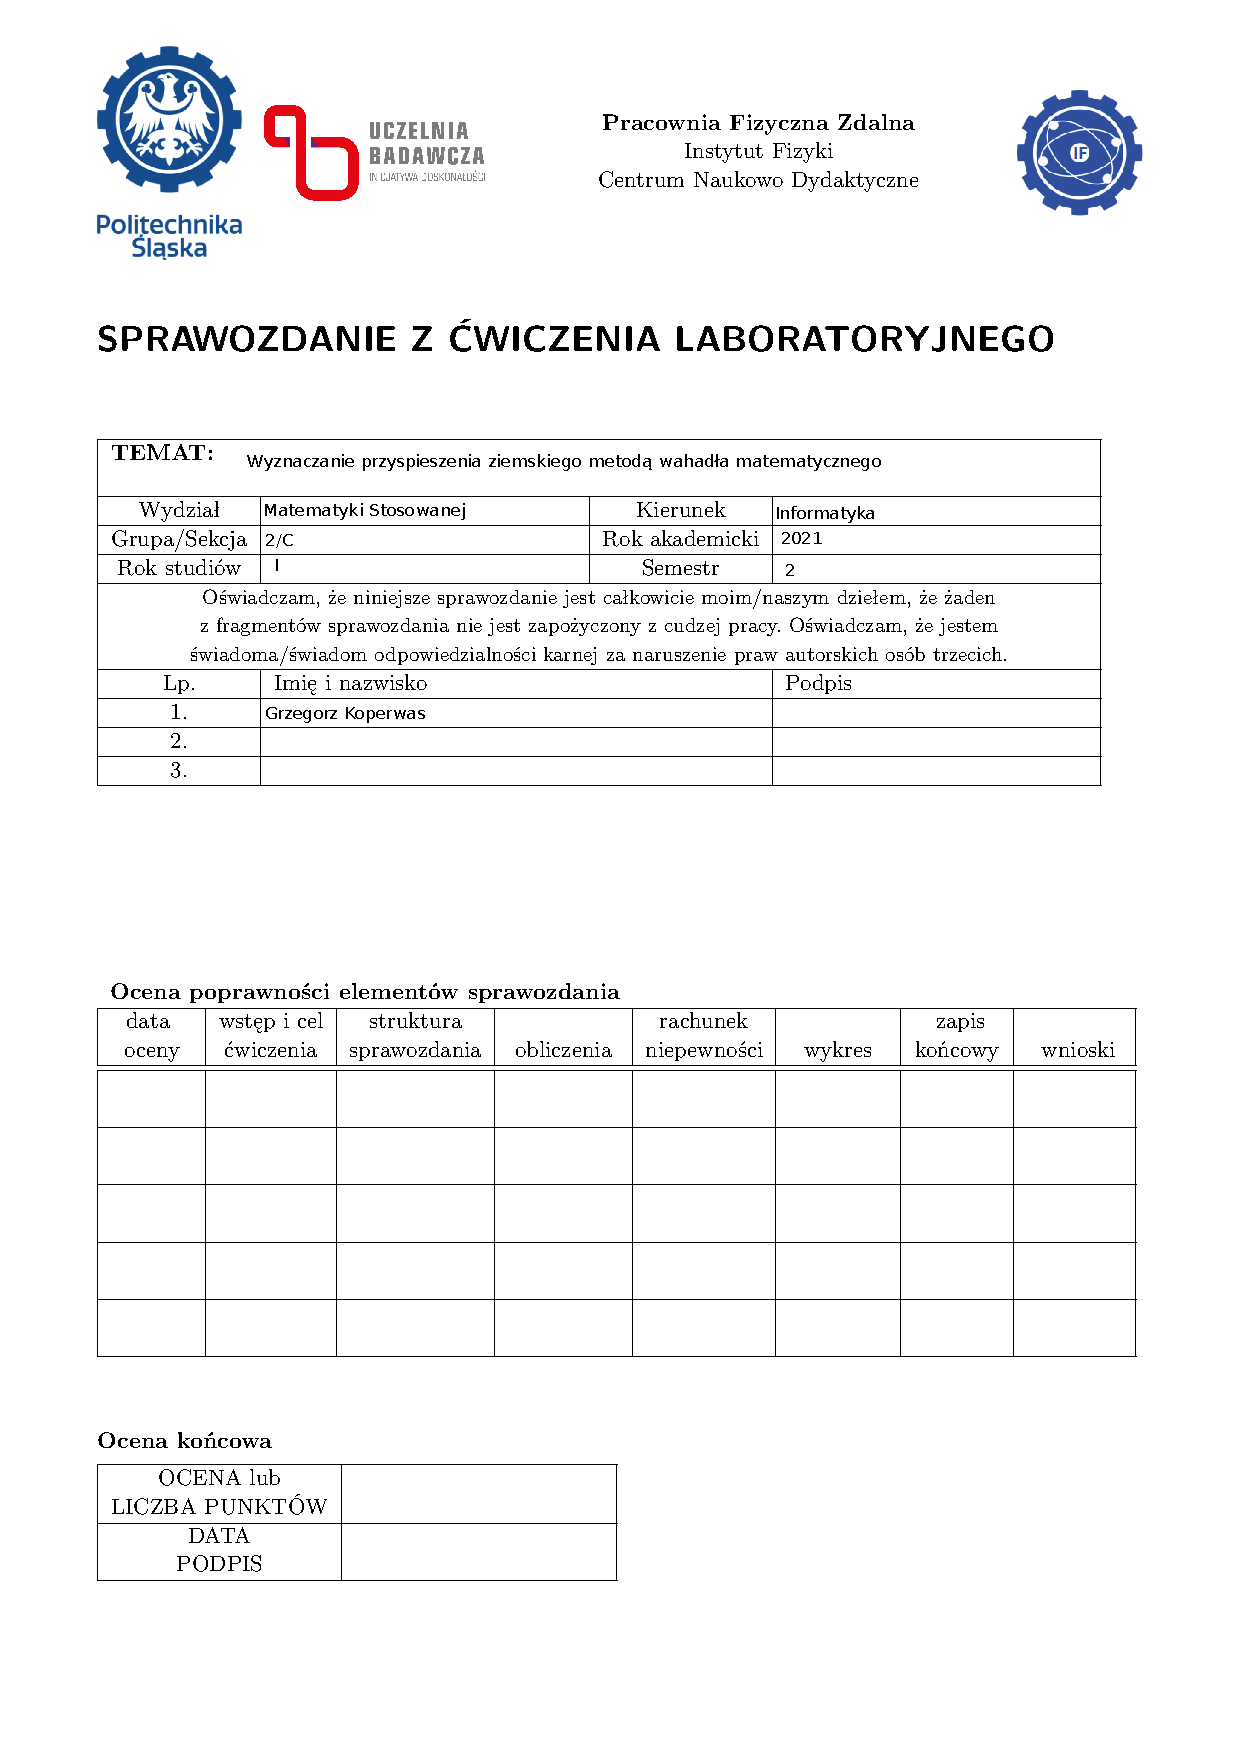
\includepdf[pages=-]{PFZ-StrTytulowaWyp.pdf}

\section{Wstęp teoretyczny}

Celem doświadczenia jest wyznaczenie przyspieszenia grawitacyjnego $g$ poprzez pomiar czasu w jakim wahadło wykona daną ilość cykli w zależności od jego długości.

\begin{figure}[h]
	\begin{tikzpicture}[scale = .7]
		\draw [dashed] (0, 0) -- (0, -6);
		\draw [dashed] (0, 0) -- (3, -5) [fill = black] circle [radius = .15];
		\node at (1.5, -2.25) [above] {$l$};
		\draw [->, thick] (3, -5) -- (3, -7) node [below]{$\vec{Q}$};
		\draw [->, thick] (3, -5) -- (2.25, -3.75) node [above]{$\vec{N}$};
		\draw [rotate = 270] (1, 0) arc (0:30:1);
		\node at (.18, -.6) {$\alpha$};
		\draw [rotate = 270, scale = 5.83, dashed] (1, 0) arc (0:30:1);
		\draw ( 0, -5 ) -- ( 3, -5 );
		\node at (1.5, -5) [above] {$x$};
		\node at (1.5, -5.7) [above] {$s$};
	\end{tikzpicture}
	\centering
	\footnotesize{
		\begin{itemize}
			\item $Q$ - ciężar
			\item $N$ - naciąg
		\end{itemize}
	}
	\caption{Wahadło w stanie największego wychylenia}
	\label{rys:wahadło}
\end{figure}

Wahadło matematyczne składa się z ciężarka, (Na rysunkach \ref{rys:wahadło} oraz \ref{rys:wahadło_siły} oznaczony jest jako kropka), który porusza się po łuku (jego długość to $s$).

Na potrzeby naszego eksperymentu rozważamy małe drgania wahadła, gdzie $\alpha < 7\stopnie$, zatem możemy założyć\cite{teoria:pw}:
\begin{equation}
	\sin \alpha \approx \alpha
\end{equation}\label{eq:smallAngle}

\begin{figure}[h]
	\begin{tikzpicture}[scale = .7]
		\draw [fill = black] (0,0) circle [radius = 0.15];
		\draw [->, thick] (0,0) -- (0, -4) node [below]{$\vec{Q}$};
		\draw [->, thick, rotate = 30] (0,0) -- (0, -3.46) node [below]{$\vec{Q_1}$};
		\draw [->, thick, rotate = -60, scale= 0.5] (0,0) -- (0, -4) node [below]{$\vec{Q_2}$};
		\draw [->, thick, rotate = 210] (0,0) -- (0, -3.46) node [above]{$\vec{N}$};
		\draw [rotate = 270, scale = 1.5](1,0) arc (0:30:1);
		\node at (.27,-.9){$\alpha$};
		\draw [dashed, thin, rotate = -60](0,0) arc (0:-30:12);
	\end{tikzpicture}
	\centering
	\footnotesize{
		\begin{itemize}
			\item $Q$ - ciężar
			\item $N$ - naciąg
		\end{itemize}
	}
	\caption{Rozkład sił na wahadle}
	\label{rys:wahadło_siły}
\end{figure}

Na rysunku \ref{rys:wahadło_siły} widzimy iż siła $\vec{Q_1}$ jest równoważona przez siłę $\vec{N}$, zatem siła $\vec{Q_2}$ jest siłą wypadkową.

\begin{align*}
	\vec{Q}             & = m\vec{g}                                                             \\
	\left|Q_2 \right|   & = mg\sin{\alpha} = mg\frac{x}{l}, \quad \text{Z (\ref{eq:smallAngle})} \\
	\left| Q_2  \right| & \approx mg \frac{s}{l}
\end{align*}

Siła $\vec{Q_2}$ jest zwrócona do środka, zatem:

\begin{equation*}
	Q_2 = - \frac{mg}{l}s
\end{equation*}

Siła ta jest zależna od wychylenia wahadła, zatem jest ona siłą sprężystą\cite{teoria:force} w formie $F = -kx$, gdzie:
\[k = \frac{mg}{l}, \quad x = s\]

Zatem układ wykonuje ruchy harmoniczne, gdzie okres drgań $T$ jest dany wzorem:

\begin{align*}
	T & = 2 \pi \sqrt{\frac{m}{k}} = 2 \pi \sqrt{\frac{m}{\frac{mg}{l}}} = \\
	  & = 2 \pi \sqrt{\frac{l}{g}}
\end{align*}

Następnie wyliczamy z wzoru $g$:

\begin{align*}
	T^2 & = 4 \pi^2 \cdot \frac{l}{g} \\
	g   & = \frac{4 l \pi^2 }{T^2}
\end{align*}

Na potrzeby sprawozdania obliczymy $g$ jako nachylenie wykresu liniowego:

\begin{align*}
	T^2               & = 4 \pi^2 \cdot \frac{l}{g} \\
	T^2\left(l\right) & = \frac{4 \pi^2}{g} \cdot l
\end{align*}

Gdzie nachylenie wykresu $T^2 \left(l\right)$ to $\frac{4 \pi^2}{g}$.

\section{Wyniki pomiarów:}

\begin{table}[h]
	\centering
	\begin{tabular}{|l|l|l|l|l|l|}
		\hline
		Długość wahadła  & \multicolumn{5}{c|}{czas 10 okresów [s] $\pm 0,01s$}                                             \\
		{[cm] $\pm 0,5cm$} & $t_{r1}$                                             & $t_{r2}$ & $t_{r3}$ & $t_{r4}$ & $t_{r5}$ \\\hline
		216,0            & 29,93                                                & 29,68    & 29,61    & 30,66    & 29,68    \\\hline
		193,5            & 28,08                                                & 28,15    & 28,13    & 28,59    & 28,00    \\\hline
		182,5            & 27,07                                                & 26,86    & 27,06    & 27,34    & 26,91    \\ \hline
		174,5            & 26,37                                                & 26,25    & 26,77    & 26,64    & 26,52    \\ \hline
		155,0            & 24,71                                                & 24,94    & 24,94    & 25,68    & 24,66    \\ \hline
		143,0            & 24,21                                                & 23,75    & 23,74    & 23,98    & 23,78    \\ \hline
		133,0            & 23,14                                                & 23,14    & 23,04    & 24,04    & 23,23    \\ \hline
		115,0            & 21,28                                                & 22,41    & 21,52    & 21,29    & 21,89    \\ \hline
		97,5             & 19,66                                                & 19,79    & 19,54    & 19,59    & 19,75    \\ \hline
		80,0             & 17,55                                                & 18,06    & 18,43    & 17,82    & 17,84    \\\hline
	\end{tabular}
	\caption{Wyniki pomiarów}
\end{table}

\begin{table}[h]
	\centering
	\footnotesize
	\begin{tabular}{|l|l|l|l|l|l|l|l|l|l|}
		\hline
		Długość wahadła    & \multicolumn{5}{c|}{długość okresu [s] $\pm 0,01s$} & Średni okres & Odchylenie & $T^2$ & $u(T^2)$                                                        \\
		{[cm] $\pm 0.5cm$} & $t_1$                                               & $t_2$        & $t_3$      & $t_4$ & $t_5$    & T[s] $\pm 0.01s$ & Standardowe [s] & [$s^2$] &       \\\hline
		216,0              & 2,99                                                & 2,97         & 2,96       & 3,07  & 2,97     & 2,99             & 0,022           & 8,95    & 0,044 \\\hline
		193,5              & 2,81                                                & 2,82         & 2,81       & 2,86  & 2,80     & 2,82             & 0,012           & 7,95    & 0,024 \\\hline
		182,5              & 2,71                                                & 2,69         & 2,71       & 2,73  & 2,69     & 2,70             & 0,010           & 7,32    & 0,019 \\\hline
		174,5              & 2,64                                                & 2,63         & 2,68       & 2,66  & 2,65     & 2,65             & 0,011           & 7,03    & 0,021 \\\hline
		155,0              & 2,47                                                & 2,49         & 2,49       & 2,57  & 2,47     & 2,50             & 0,021           & 6,24    & 0,042 \\\hline
		143,0              & 2,42                                                & 2,38         & 2,37       & 2,40  & 2,38     & 2,39             & 0,010           & 5,71    & 0,021 \\\hline
		133,0              & 2,31                                                & 2,31         & 2,30       & 2,40  & 2,32     & 2,33             & 0,021           & 5,44    & 0,042 \\\hline
		115,0              & 2,13                                                & 2,24         & 2,15       & 2,13  & 2,19     & 2,17             & 0,024           & 4,70    & 0,049 \\\hline
		97,5               & 1,97                                                & 1,98         & 1,95       & 1,96  & 1,98     & 1,97             & 0,005           & 3,87    & 0,011 \\\hline
		80,0               & 1,76                                                & 1,81         & 1,84       & 1,78  & 1,78     & 1,79             & 0,017           & 3,22    & 0,033 \\\hline
	\end{tabular}
	\caption{Przetworzone wyniki pomiarów}
\end{table}
\clearpage
\section{Wykres}

\begin{figure}[h]
	\centering
	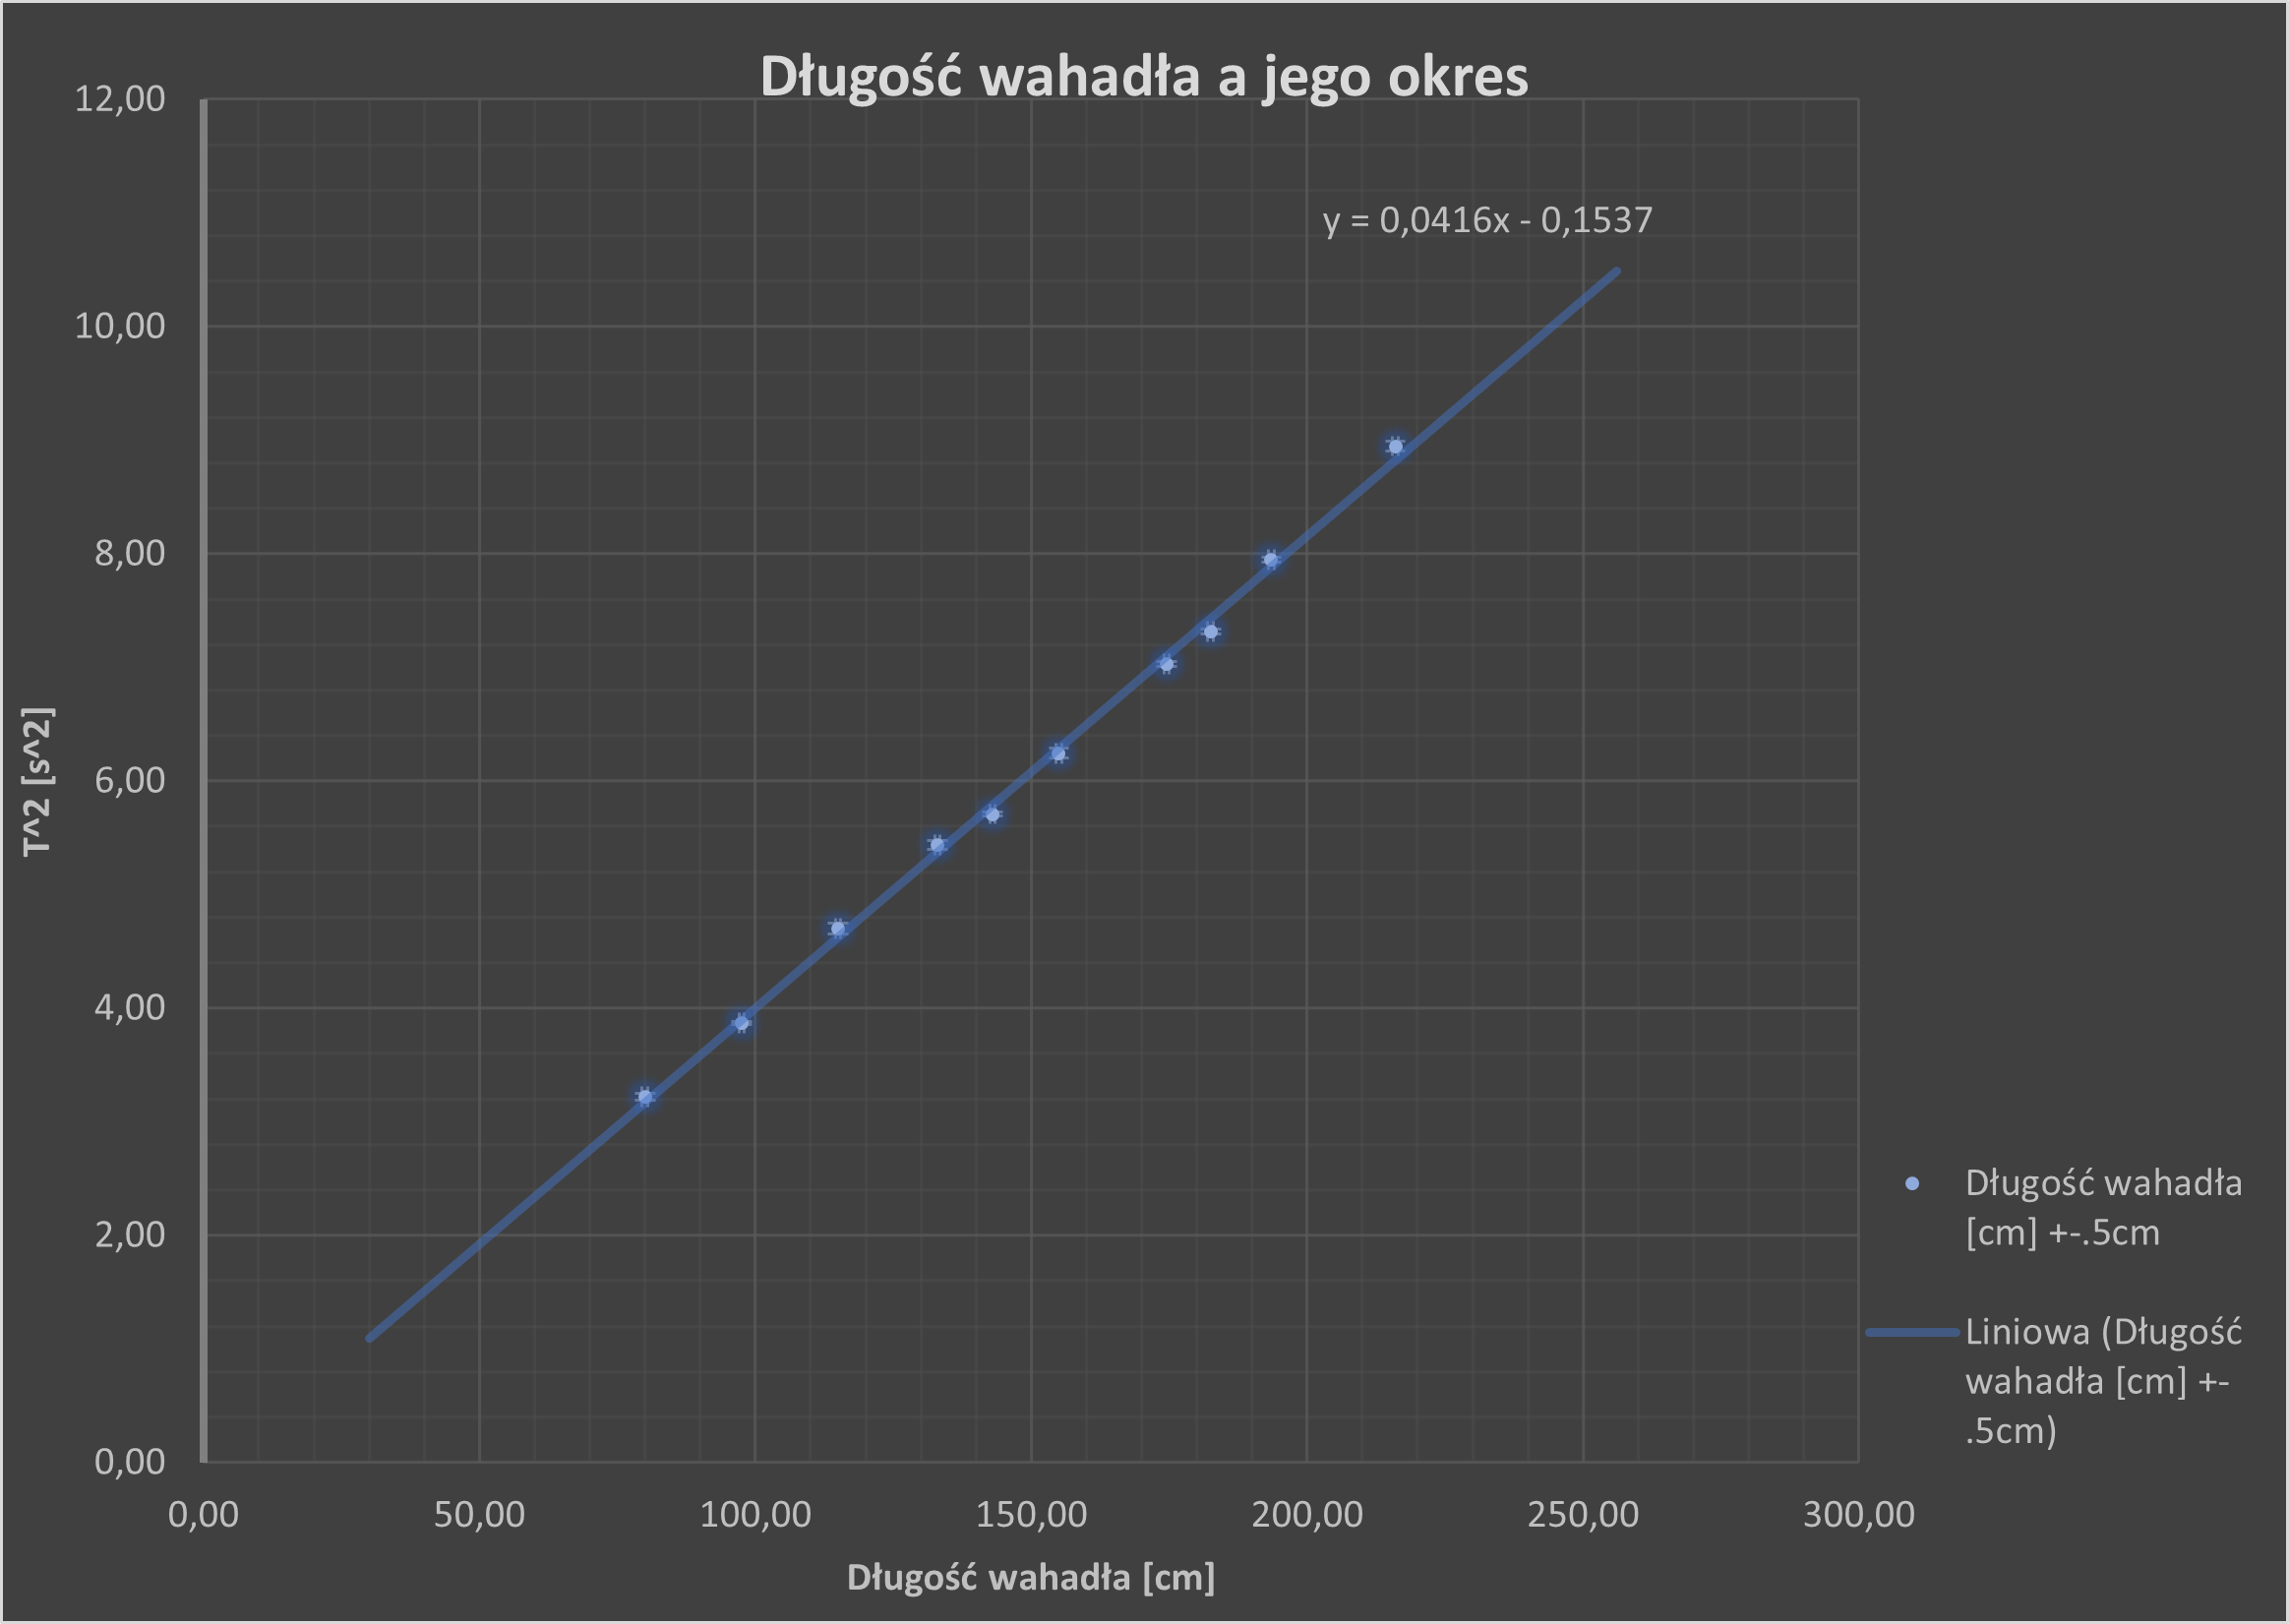
\includegraphics[width=\linewidth, keepaspectratio]{Wykres.png}
	\caption{Wykres $T^2$ od $l$}\label{wykt2}
\end{figure}

Słupki błędów na wykresie na rysunku \ref{wykt2} są małe\footnote{
		Dla  podziałki długości 10cm, niepewność to $\frac{1}{20}$ podziałki, podobnie dla podziałki $T^2$, która jest równa $0,4 s^2$, gdzie niepewności są rzędu maksymalnie $\frac{1}{10}$ wielkości podziałki.
	}, należy bardzo przybliżyć sobie widok\footnote{Z powodu ograniczeń w programie Excel spróbuje w następnych sprawozdaniach użyć innego programu, np. Matplotlib czy Logger Pro.}.
Z wykresu odczytujemy:

\begin{itemize}
	\item $a = 0,042 \frac{s^2}{cm};\; u\left(a\right) = 0,00065 \frac{s^2}{cm}$
	\item $b = -0,15 s^2;\; u\left(b\right) = 0,10 s^2$
\end{itemize}

\section{Wnioski:}

Według metody $g$ obliczamy ze wzoru:

\[ \frac{4\pi^2}{a \cdot 100} = g \]

Zatem dla $a = 0,41$ dostajemy wartość $g = 9,50$. Niepewność obliczmy ze wzoru:

\[ \frac{g}{a} \cdot u\left(a\right) = u\left(g\right) \]

Zatem $u\left(g\right) = 0,15$.

Ostatecznie:

\[ g = 9,50 \frac{m}{s^2};\;  u\left(g\right) = 0,15 \frac{m}{s^2} \]

\subsection*{Porównanie z wartościami tablicowymi}

$g_f$ możemy obliczyć ze wzoru\cite{wzor}:

\[g_f \approx 9,780318 \left(1 + 0,0053024 \sin^2 \alpha - 0,0000058 \sin^2 2\alpha\right) - 3,086 \cdot 10^{ -6} h\]

Gdzie
\begin{itemize}
	\item $\alpha = 50,36\stopnie$ - szerokość geograficzna miejsca pomiaru
	\item $h = 278m$ - wysokość Gliwic nad poziomem morza.
\end{itemize}

Dla Gliwic $g_f = 9,81$. Zatem:
\begin{align*}
	\left| g - g_f \right|  & = \left| 9,50 - 9,81 \right| = 0,31 \\
	2 \cdot u\left(g\right) & = 2 \cdot 0,15 = 0,30               \\
	0,31\,                  & \not\leq 0,30
\end{align*}

Z czego wynika iż wartość otrzymana nie jest zgodna z wartością tablicową.

\subsection*{Możliwe źródła błędów}

Głównym źródłem błędów było nieprzykładne mierzenie czasu okresów, lepsza metoda pomiarowa lub większa liczba pomiarów pozwoliłaby na ograniczenie błędów przypadkowych. Zastosowanie metody pomiaru okresu za pomocą kamery i analizy materiału video było by dokładniejsze, mimo teoretycznie mniejszej dokładności ($\frac{1}{30}$ sekundy\footnote{Dla kamery mogącej nagrywać tylko w 30 klatkach na sekundę} zamiast $0,01$ dla stopera zastosowanego w doświadczeniu), pozwoliła by ona wyeliminować błąd wynikający z refleksu prowadzącego doświadczenie.

\bibliographystyle{alpha}
\bibliography{Sprawozdanie}
\end{document}
